\begin{frame}
\frametitle{Inertial particles and turbulence}
	% Applications
%    \begin{textblock*}{90mm}[0,0](-5mm,-2mm)
%    \textcolor{myred}{\textbf{Many fields of application}}
%    \begin{itemize}
%        \item \textbf{Natural} : plankton, marine snow, rain, pollutants
%        \item \textbf{Industrial} : chemical reactors, combustion chambers
%    \end{itemize}
%    \end{textblock*}
    
\begin{textblock*}{30mm}[0,0](0mm,2mm)
	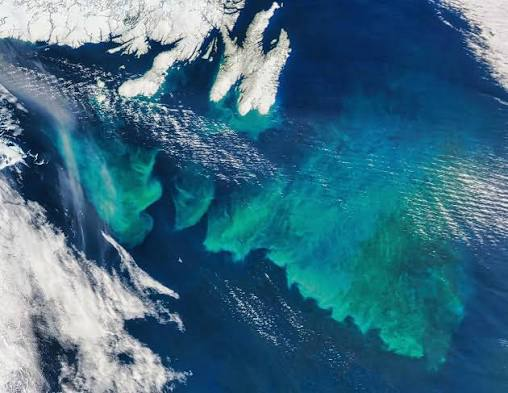
\includegraphics[width = \textwidth]{images.jpeg}
\end{textblock*}

\begin{textblock*}{70mm}[0,0](0mm,45mm)
	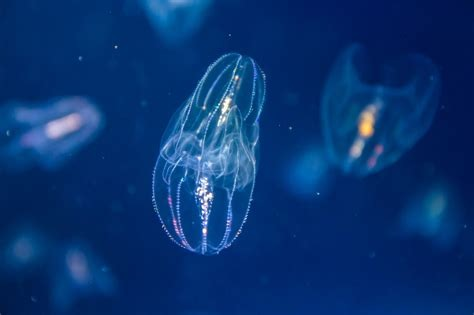
\includegraphics[clip,trim=0 0 0 0,width = .45\textwidth]{plankton.jpg}\\[2pt]
	\footnotesize{Increase meeting\\probabilities}
\end{textblock*}

\begin{textblock*}{30mm}[0,0](42mm,-1mm)

\end{textblock*}
\begin{textblock*}{40mm}[0,0](40mm,14mm)
\textcolor{myred}{{\textbf{Cluster formation}}}\\[4pt]
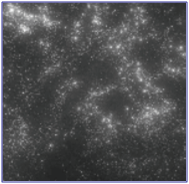
\includegraphics[width=30mm]{inertial.png}
\end{textblock*}
\begin{textblock*}{40mm}[0,0](39mm,62mm)
	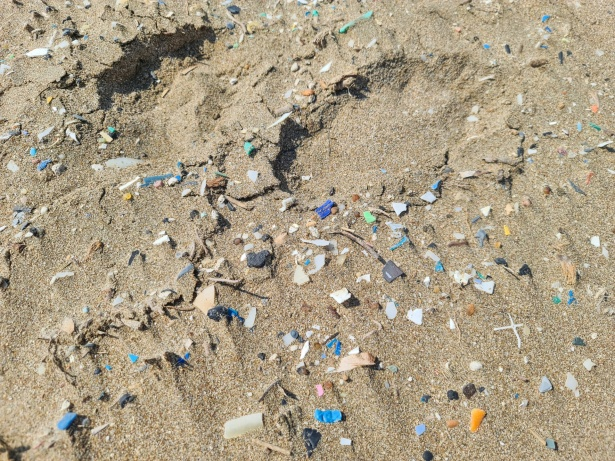
\includegraphics[clip, trim=0 30 0 150 , width = \textwidth]{microplastics-on-the-beach-1662635283OyR.jpg}
\end{textblock*}

\begin{textblock*}{30mm}[0,0](83mm,0mm)
	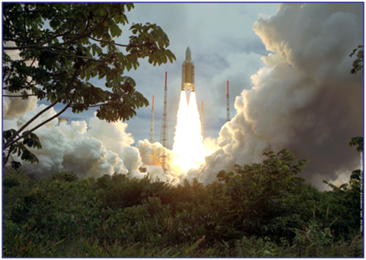
\includegraphics[width = \textwidth]{Fusee.png}\\[2pt]
	\footnotesize{Stoichiometric proportion}
\end{textblock*}
\begin{textblock*}{30mm}[0,0](83mm,35mm)
	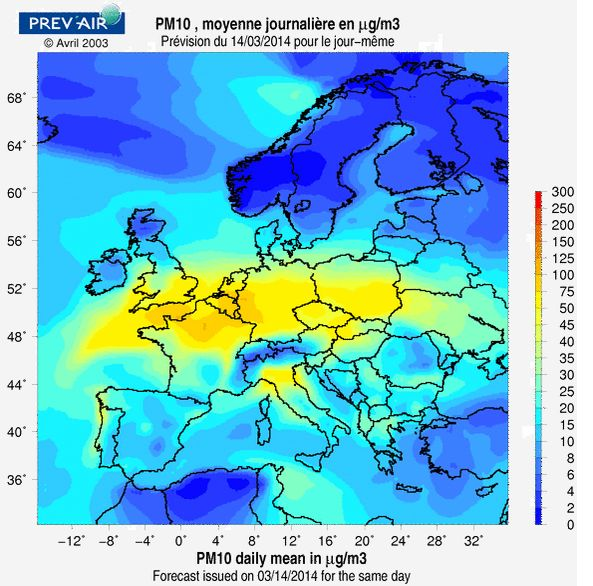
\includegraphics[clip,trim=30 45 58 55,width = \textwidth]{Carte_PM10_Europe_20140314.JPG}\\[2pt]
	\footnotesize{Sanitary thresholds}
\end{textblock*}
%	{%
%		\setlength{\fboxsep}{0pt}%
%		\setlength{\fboxrule}{1pt}%
%		\fbox{\includegraphics[options]{image}}%
%	}%


\end{frame}